% !TEX root = ../../Main.tex
\fancychapter{Background}
\label{Chapter:Background}

This chapter covers the background needed to follow the rest of this thesis. It starts with financial markets, and in particular with the Forex market, how trading works there and what it costs. It then covers neural networks and reinforcement learning, the two fields of machine learning this work uses. It ends with Deep Reinforcement Learning, which joins the two, and with the algorithm used in this work.

% !TEX root = ../../Main.tex
\section{Financial Markets and Trading}

Financial markets move capital between those who have it and those who need it. In these markets, participants trade assets, hedge risk and raise funds. Each type of market has a different purpose, and \Cref{Tables:FinancialMarkets} summarises the main ones. The markets are connected. A movement in one often passes on to the others, so none of them is studied on its own. The market participants themselves set the prices. They range from private investors to banks and investment funds. Regulators set the rules that these participants must follow. Electronic platforms and algorithmic execution have opened the markets to more participants and have made prices adjust faster \cite{brandimarte_introduction_2018}.

% !TEX root = ../Main.tex
\begin{table}[htb!]
\centering
\footnotesize
\caption{Summary of Financial Markets and their Economic Role \cite{brandimarte_introduction_2018}.}
\label{Tables:FinancialMarkets}
\begin{tabularx}{\textwidth}{@{}lXl@{}}
\toprule
\textbf{Market} & \textbf{Economic Role} & \textbf{Asset Examples} \\
\midrule
Equity Market & Raising capital by trading company shares. & Stocks, Equities \\
\addlinespace
Bond Market & Debt financing, where entities borrow from investors. & Government and Corporate Bonds \\
\addlinespace
Commodities Market & Trading basic raw materials and agricultural goods. & Oil, Gold, Wheat \\
\addlinespace
Forex Market & Currency exchange for international trade. & USD, EUR, JPY, GBP \\
\addlinespace
Derivatives Market & Trading contracts for hedging or speculation. & Futures, Options, Swaps \\
\addlinespace
Indices Market & Combining and tracking the performance of a market or sector. & S\&P 500, NASDAQ \\
\addlinespace
Cryptocurrency Market & Exchanging digital currencies. & Bitcoin, Ethereum \\
\bottomrule
\end{tabularx}
\end{table}

\subsection{Forex Market: Characteristics and Significance}

The Foreign Exchange market, or Forex market, is where currencies are exchanged. It is the largest financial market by turnover. In April 2025 it traded 9.6 trillion US dollars per day on average, 28\% more than the 7.5 trillion recorded three years earlier. It trades continuously across time zones, because the banks and institutions that quote its prices are spread around the world. Spot transactions, the instrument traded in this work, make up 3 trillion of that daily total. The US Dollar is on one side of 89.2\% of all trades, and the ten most traded currency pairs all include it \cite{bis_otc_2025}. Prices react to interest rate decisions, economic releases and political events. Participants normally trade with leverage. Leverage allows a position much larger than the capital deposited, and it scales profits and losses in the same proportion. Its market depth, its continuous operation, its sensitivity to news and the routine use of leverage make it suitable for automated trading. The same properties make it hard to model. Its behaviour is noisy and non-stationary, which means that its statistical properties change over time. This is why adaptive, data-driven strategies are of interest \cite{donnelly_art_2019}.

\subsection{Forex Trading: Fundamental Concepts and Operation}

Trading a currency pair means buying one currency and selling another at the same time. Buying the EUR/USD pair means buying Euros and selling US Dollars, expecting that the Euro will strengthen against the US Dollar. This work uses the seven major currency pairs: EUR/USD, USD/JPY, GBP/USD, AUD/USD, USD/CHF, NZD/USD and USD/CAD. They are built from the Euro (EUR), US Dollar (USD), Japanese Yen (JPY), British Pound (GBP), Australian Dollar (AUD), Swiss Franc (CHF) and New Zealand Dollar (NZD). Every one of them has the US Dollar on one side. Deciding whether to buy or sell a pair comes down to predicting the strength of one currency relative to the other \cite{donnelly_art_2019}.

A position is the exposure a trader holds in a pair. It is the amount of the pair that the trader has bought or sold and not yet closed. A long position makes money when the pair rises and loses money when it falls. A short position does the opposite. A currency pair is a ratio between two currencies, so short selling is as natural as buying and needs no borrowing. In equity markets this is not the case. Positions are opened and closed with orders. A market order is executed at once, at the price quoted at that moment. A limit order is executed only at a given price or better. A stop order is executed once the price passes a given level. Two stop orders are often attached to an open position. A stop loss closes the position when the loss reaches a chosen level. A take profit closes it when a target is reached.

Forex trading takes place in a decentralised market that works worldwide. There is no single exchange where all trades happen. Instead, trades are handled by a network of market makers and brokers. The market makers are mainly banks, and the market between them is known as the interbank market. Interbank trades are large, and most of them are made by institutions such as multinational companies and large hedge funds. Retail traders take part through brokers, who have access to that network and act as intermediaries. Market makers and brokers always quote two prices. The bid price is the price at which they will buy the pair. The ask price is the price at which they will sell it. The difference between the two is the spread. Without a central trading venue, one might expect the market to be poorly regulated. However, competition between market makers keeps their quoted prices close to one another and keeps spreads narrow \cite{donnelly_art_2019}.

Traders look at prices on charts, and the candlestick chart is the standard type. A candlestick chart is made of candlesticks. Each one shows how the price moved over a period of time, which can be anything from minutes to years. A tick is a single update of the quoted price. It is published whenever a market maker changes its bid or its ask. The name comes from its shape, which looks like a candle with a wick at both ends. Each candlestick shows the opening price (O), the highest price (H), the lowest price (L) and the closing price (C) of its period (see \Cref{Figure:CandlestickChart}). The colour of the candlestick shows the direction of the move. A lighter shade means the price went up, and a darker shade means it went down. This lets traders see the direction of the market quickly, just by looking at the chart. Candlestick charts do not show volume (V), which is normally drawn separately below the price. Forex has no central venue, so there is no consolidated record of traded size. Brokers report tick volume instead, which is the number of quote updates in the period. This work uses tick volume throughout \cite{rhoads_candlestick_2022}.

\begin{figure}[htb!]
\centering
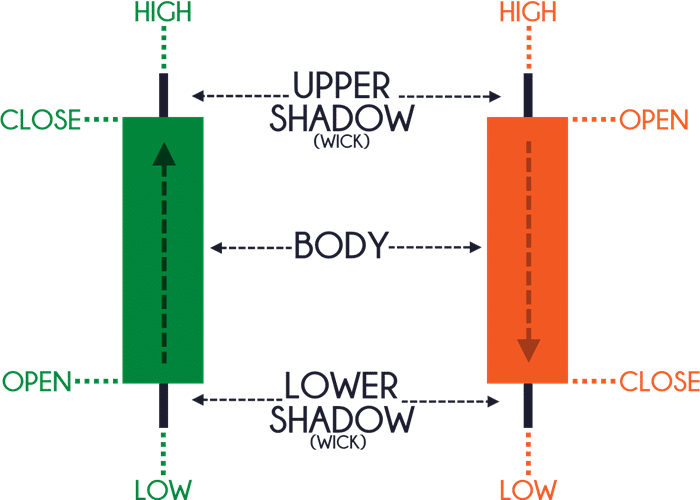
\includegraphics[width=0.4\textwidth]{Images/CandlestickChart.png}
\caption{Candlesticks showing upward (bullish) and downward (bearish) movements respectively \cite{teo_candlestick_nodate}.}
\label{Figure:CandlestickChart}
\end{figure}

This work uses tick data as its main record, because it has the finest resolution the broker provides. Whenever a coarser view is needed, it computes from the ticks the opening, highest, lowest and closing prices and the tick volume, called OHLCV data for short \cite{rhoads_candlestick_2022}. Indicators computed from that data give the model more context, as described below.

\subsection{Forex Costs: Spreads, Commissions and Overnight Financing}

Trading is not free, and its costs are large compared with the profit a single position can make. Three costs apply in Forex, and each is charged separately from the others. Prices are quoted in units that depend on the pair. A pip is the fourth decimal place of the quote for most pairs, or the second for pairs quoted against the Japanese Yen. A point is one tenth of a pip. It is the smallest price increment a broker quotes. The size of a position is given in units of the base currency, the first currency of the pair, and one standard lot is $100{,}000$ units. For a position of volume $q$ at price $p$, the notional value, which is the value of the position in the quote currency (the second currency of the pair), is

\begin{equation}
V = q \cdot p
\end{equation}

The \textbf{spread} is the first cost. It is an implicit cost, paid through the price. A position is opened at the ask and closed at the bid, so a full round trip, opening and then closing, crosses the spread once. For a position of volume $q$, the cost is

\begin{equation}
C_{spread} = (p_{ask} - p_{bid}) \cdot q
\label{Equation:SpreadCost}
\end{equation}

The spread is not constant. It widens when liquidity falls, around economic releases and at the daily rollover. A strategy tested with a fixed spread is therefore tested on a market that does not exist in practice.

The \textbf{commission} is the second cost, and it is an explicit cost. Some accounts quote the raw interbank spread. On these accounts the broker makes its money through a commission charged on the traded volume, instead of through a wider spread. If the commission is given as a number of points $c$, and $s_{point}$ is the size of one point, the cost of a position of volume $q$ is

\begin{equation}
C_{commission} = c \cdot s_{point} \cdot q
\label{Equation:CommissionCost}
\end{equation}

The spread and the commission are separate costs, and a trader pays both. On a raw-spread account, treating the spread as if it already included the commission makes trading look cheaper than it is.

The \textbf{swap}, or overnight financing, is the third cost. It comes from the interest rate differential between the two currencies of the pair. It is charged when a position is still open at the daily rollover, the moment when the trading day ends. On one day of the week the charge is multiplied, to cover the weekend. Depending on the direction of the position and the sign of the differential, the swap can be a cost or a credit. Some account types remove it completely, so that clients can avoid interest for religious reasons. These are known as swap-free accounts. Finally, leverage decides how much capital a position needs. With leverage $L$, the margin, which is the capital set aside for a position of notional value $V$, is

\begin{equation}
M = \frac{V}{L}
\end{equation}

Leverage does not change the profit or loss of a position. It only changes the capital set aside for it. So leverage affects the return of the account, and the return of the trade stays the same. These costs are not the same on every type of account. Choosing the account is therefore part of designing a strategy. A raw-spread account quotes the interbank spread with no markup and makes its money through the commission. This makes the total cost of a position lower. It also makes the cost explicit, which is more useful. The implicit part of the cost is reduced to the market spread, and the rest is a published rate. A swap-free account charges no overnight financing at all. An account with both features suits a strategy that holds positions for days. Such a strategy pays the spread and the commission only a few times per position, but it would otherwise pay financing for every night the position stays open. This work is evaluated on an account that has both features. The spread and the commission are therefore the only costs applied, and the financing cost is exactly zero, so it does not need to be estimated.

\subsection{Financial Analysis: Main Types and Formulas}

Representing the data is one half of the problem. The other half is analysing it to decide what to trade. Financial analysis is usually divided into three types \cite{lim_handbook_2015}:

\begin{itemize}
\item \textbf{Fundamental Analysis}: studies the economic factors that affect currency prices. These include GDP growth, employment rates, interest rates and monetary policy, which help to predict currency trends from the economic health of a country. However, much of this data is qualitative. This makes it hard to use in computer models, which work best with structured numerical input.
\item \textbf{Sentiment Analysis}: tries to measure the mood of the market by analysing news, market commentary and similar qualitative data. It aims to measure how the shared emotions of traders affect market trends. It is complex and needs advanced natural language processing, so it is harder to include in a model.
\item \textbf{Technical Analysis}: analyses past OHLCV data to predict future market movements. It assumes that past market behaviour will repeat itself, so patterns or measures found in current data can predict future movements. It is preferred because its results are numbers, which complex machine learning models can use.
\end{itemize}

Of the three, this work uses technical analysis. It produces numerical series directly from price data, so a model can use them without any further interpretation. Technical analysis is divided into indicators and candlestick patterns. Indicators are measures calculated from past market data, created mainly by mathematicians and economists. They give a numerical view of how the market moves. They are usually grouped into four main types \cite{lim_handbook_2015}:

\begin{itemize}
\item \textbf{Trend Indicators}: Used to find the main direction of the market by filtering out market noise. See \Cref{Tables:TrendIndicators} for details of frequently used indicators.
\item \textbf{Momentum Indicators}: Used to measure the momentum of a trend, whether it is strong or weak, and whether a reversal is expected. See \Cref{Tables:MomentumIndicators} for details of frequently used indicators.
\item \textbf{Volume Indicators}: Used to look at the trading volume, which gives clues about the strength of a price movement. See \Cref{Tables:VolumeIndicators} for details of frequently used indicators.
\item \textbf{Volatility Indicators}: Used to measure the level of uncertainty or risk that comes with the volatility of the price. See \Cref{Tables:VolatilityIndicators} for details of frequently used indicators.
\end{itemize}


The four tables list indicators in common use. They do not describe the contents of any one system. The framework built for this work implements the moving average family and the crossovers between its members, the Rate of Change, the Moving Average Convergence Divergence, the Average True Range, the Realised Volatility and the Efficiency Ratio. It implements no volume indicators. The tick volume a Forex broker reports counts quote updates, not traded size, and this limits what those indicators can measure. Ten instances of the implemented set form the observation the agent receives. They are listed in \Cref{Chapter:Implementation}. Candlestick patterns work differently. They do not compute a value. They describe shapes, formed by one or more candlesticks, that traders link to a change in behaviour \cite{rhoads_candlestick_2022}. Such patterns can be encoded as numbers and given to a model in the same way as an indicator \cite{jansen_machine_2020}. This work does not use them. The observation is built from indicators only.

\subsection{Performance Measurement: Returns, Risk and Ratios}
\label{Section:PerformanceMeasurement}

A trading strategy is judged by what it earns and by the risk it takes to earn it. A single return figure is therefore not enough to compare two strategies. The measures below are the ones reported in \Cref{Chapter:ExperimentalResults}. They are defined on an equity series, which is the value of the account over time. They therefore apply without change to a portfolio of several strategies. They are then computed on the combined equity of the portfolio, and not on each strategy separately. This matters because the risk of a portfolio depends on how its parts move together, and not only on the risk of each part.

The total return over a period compares the final and the initial equity $E$ of the account:

\begin{equation}
R = \frac{E_{final} - E_{initial}}{E_{initial}}
\end{equation}

Periods differ in length, so returns are annualised, that is, converted to a yearly rate, before they are compared. With a duration $\Delta t$ in seconds and a year of $365$ days,

\begin{equation}
R_{annual} = (1 + R)^{\frac{365 \cdot 86400}{\Delta t}} - 1
\label{Equation:AnnualizedReturn}
\end{equation}

Risk is measured in two ways. The first is volatility, which is the standard deviation of returns, annualised by the rate at which the strategy trades. The second is drawdown. At any moment, the drawdown is the distance between the current equity and the highest equity reached so far:

\begin{equation}
D(t) = \frac{E(t) - \max_{s \leq t} E(s)}{\max_{s \leq t} E(s)}
\label{Equation:Drawdown}
\end{equation}

The maximum drawdown is the worst value of $D(t)$ over the period. It is the largest loss from a peak that an investor would have suffered. The mean drawdown is the average of $D(t)$. It shows how far below its peak the account is on a typical day, instead of at its worst moment. Four ratios combine return and risk. All of them divide an annualised excess return, which is the return above the risk-free rate, by a measure of risk. They differ only in the measure of risk they use. The absolute value of that measure is used, because a drawdown is negative under the definition above. With $R_f$ as the risk-free rate,

\begin{equation}
\text{Ratio} = \frac{R_{annual} - R_f}{\left| \text{risk} \right|}
\label{Equation:RiskRatio}
\end{equation}

The \textbf{Sharpe ratio} \cite{sharpe_sharpe_1994} uses the annualised volatility, so it penalises upward and downward moves equally. The \textbf{Sortino ratio} \cite{sortino_performance_1994} uses the downside volatility instead, computed from negative returns only. The argument is that an investor does not mind upside variability. The \textbf{Calmar ratio} uses the maximum drawdown, so it measures return against the worst loss suffered. The \textbf{Sterling ratio} uses the mean drawdown. This makes it less sensitive to a single bad period, and closer to what holding the strategy is like on a typical day. The Calmar and Sterling ratios both have several definitions in the literature, and the ones used here follow \cite{bacon_practical_2023}. By construction, the mean drawdown is smaller than the maximum drawdown. So, for a strategy with a positive excess return, the Sterling ratio is the larger of the two ratios. When the excess return is negative, the order is reversed.

\subsection{Algorithmic and Quantitative Trading}

More and more of the trading in financial markets is done by algorithms. Algorithmic trading uses computer programs to execute trades faster and in larger volume than a human can. The programs analyse large datasets, read market conditions and act on set rules. Algorithmic trading is used for pre-trade analysis, signal generation and trade execution. It is what allows institutions to run complex strategies at a large scale. Quantitative trading is a subfield of algorithmic trading. It uses mathematical and statistical models to find opportunities in market data, through the analysis of past data and through machine learning. It follows systematic rules instead of the discretionary judgement of a trader, and it needs knowledge of both finance and mathematics \cite{chan_quantitative_2021}. Together, the two have changed how markets work. They brought practices such as high-frequency trading, and they shortened the time that prices take to react to new information. They have also made machine learning central to the field. Neural networks are used to find structure in market data, and reinforcement learning is used to decide what to do with it \cite{jansen_machine_2020}. These two fields are the subject of the next sections.

% !TEX root = ../../Main.tex
\section{Neural Networks}

Machine learning covers algorithms that find patterns in data and act on them, without being programmed with the rules in advance. Tom Mitchell states the idea as follows \cite{mitchell_machine_1997}:
\begin{quote}
"A computer program is said to learn from experience E with respect to some task T and some performance measure P, if its performance on T, as measured by P, improves with experience E."
\end{quote}
The definition is useful here because it describes exactly what a trading agent does. The task is choosing a position. The performance measure is the money that position makes. The experience is the market data the agent has already seen. Neural networks, the subject of this section, are the class of models used to represent that behaviour.

\subsection{Fundamentals and History}

Neural Networks (NN) are algorithms designed for pattern recognition. They are named after the human brain, because their structure is similar to it. In the brain, a neuron receives signals through structures called dendrites and processes them in the nucleus. It then passes the result down its axon to the dendrites of nearby neurons. A neural network works in a similar way. Each node is an artificial neuron. It receives an input, processes it with a mathematical function and passes the output to the next layer of nodes. In both cases, the strength and the type of the connections between neurons decide how the network behaves \cite{goodfellow_deep_2016}. \Cref{Figure:HumanNeuronVsArtificialNeuron} illustrates these ideas.

\begin{figure}[htb!]
\centering
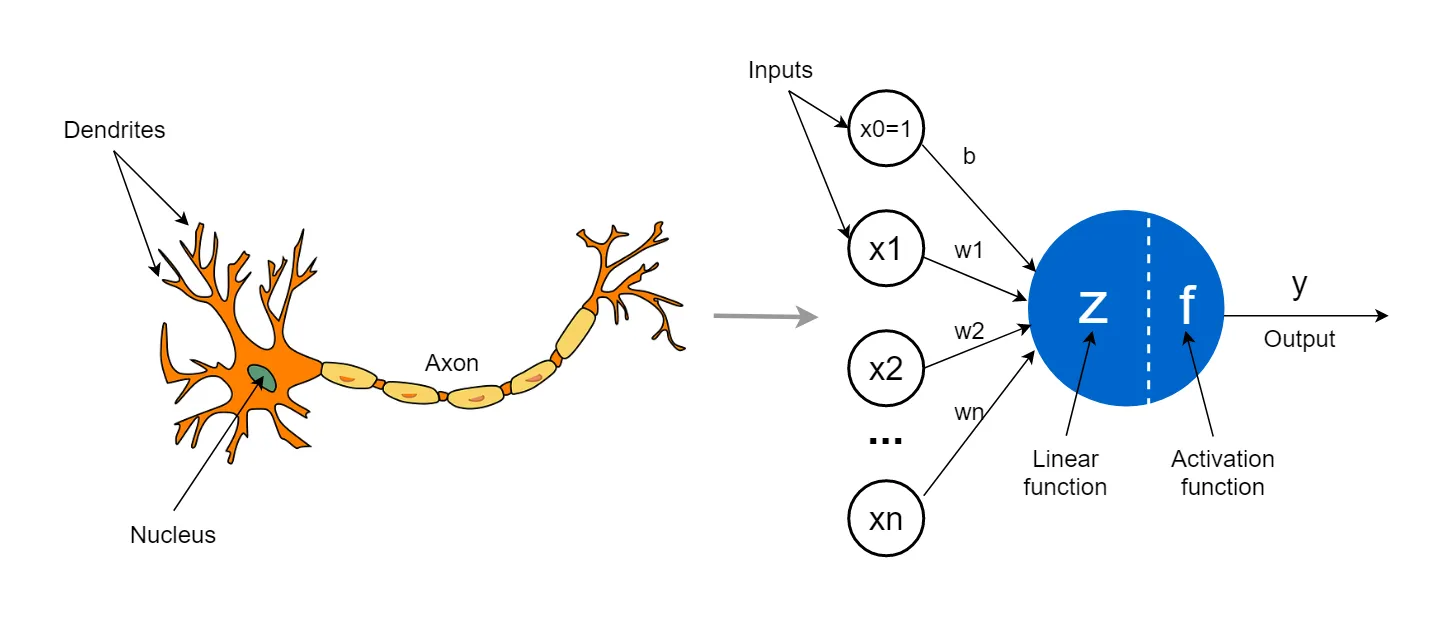
\includegraphics[width=0.7\textwidth]{Images/HumanNeuronVsArtificialNeuron.png}
\caption{Human Neuron compared to an Artificial Neuron \cite{pramoditha_human_nodate}.}
\label{Figure:HumanNeuronVsArtificialNeuron}
\end{figure}

The idea of neural networks goes back to the 1950s and the perceptron, a simple model of a biological neuron developed by Frank Rosenblatt \cite{rosenblatt_perceptron_1958}. The perceptron was the start of NN research. However, it could only learn linearly separable datasets, in which a straight line or a flat plane can separate the classes. This limit led to some periods of low interest in the field, known as ``AI winters''. A major advance came in the 1980s with the backpropagation algorithm. It allowed complex multilayer neural networks to learn patterns in datasets that are not linearly separable \cite{rumelhart_learning_1986}.

\subsection{Key Concepts and Feed-Forward}

In a neural network, the feed-forward computation in each layer \( l \) uses the output of the layer before it. For the first layer, this input \( x \) is the raw data itself. For the later layers, it is the output of the previous layer, \( h^{(l-1)}(x) \). The computation in each layer can be written as \cite{goodfellow_deep_2016}:

\begin{equation}
z^{(l)}(x) = W^{(l)} h^{(l-1)}(x) + b^{(l)}
\end{equation}

Here, the weight matrix \( W^{(l)} \in \mathbb{R}^{K_l \times K_{l-1}} \) and the bias vector \( b^{(l)} \in \mathbb{R}^{K_l} \) are used in the computation of layer \( l \). \( K_l \) is the number of neurons, or units, in layer \( l \), and \( K_{l-1} \) is the number of neurons in the previous layer \( l-1 \). For the first layer, \( W^{(1)} \in \mathbb{R}^{K_1 \times D} \), where \( D \) is the size of the input data. The activation function \( g \) is then applied to the pre-activation \( z^{(l)}(x) \in \mathbb{R}^{K_l} \) to give the activated output \( h^{(l)}(x) \in \mathbb{R}^{K_l} \) \cite{goodfellow_deep_2016}:

\begin{equation}
h^{(l)}(x) = g(z^{(l)}(x))
\end{equation}

The choice of activation function matters in two places. In the hidden layers, the function must be non-linear. A stack of linear layers is equal to a single linear transformation, so the network would gain nothing from its depth. In the output layer, the task decides the function. A bounded function is used when the output must stay within a range, and no activation is used when it does not \cite{goodfellow_deep_2016}. \Cref{Tables:ActivationFunctions} summarises the most common activation functions.

% !TEX root = ../Main.tex
\begin{table}[htb!]
\centering
\footnotesize
\caption{Summary of the most common Activation Functions \cite{goodfellow_deep_2016}.}
\label{Tables:ActivationFunctions}
\begin{tabularx}{\textwidth}{@{}lXl@{}}
\toprule
\textbf{Activation Function} & \textbf{Formula} & \textbf{Description} \\
\midrule
Linear & \( a(x) = x \) & Suitable for regression tasks. \\
\addlinespace
Sigmoid & \( \sigma(x) = \frac{1}{1 + e^{-x}} \) & Maps inputs to (0, 1), for binary classification. \\
\addlinespace
Hyperbolic Tangent & \( \tanh(x) = \frac{e^{x} - e^{-x}}{e^{x} + e^{-x}} \) & Maps inputs to (-1, 1), with stronger gradients than sigmoid. \\
\addlinespace
ReLU & \( \text{ReLU}(x) = \max(0, x) \) & Leads to sparse activation, helps gradient flow. \\
\addlinespace
Softmax & \( \text{Softmax}(z)_i = \frac{e^{z_i}}{\sum_{k=1}^K e^{z_k}} \) & Turns raw scores (logits) into probabilities, for multi-class classification. \\
\bottomrule
\end{tabularx}
\end{table}

\subsection{Learning using Backpropagation}

Neural networks learn by adjusting their weights and biases step by step, to reduce the error between the predicted outputs and the true target values. A loss function measures this error and guides the learning. The goal is to find the parameters that minimise the loss function. Different problems need different loss functions, such as mean squared error for regression tasks and cross-entropy for classification \cite{goodfellow_deep_2016}. \Cref{Tables:LossFunctions} gives their formulas.

% !TEX root = ../Main.tex
\begin{table}[htb!]
\centering
\footnotesize
\caption{Summary of the most common Loss Functions \cite{goodfellow_deep_2016}.}
\label{Tables:LossFunctions}
\begin{tabularx}{\textwidth}{@{}lXl@{}}
\toprule
\textbf{Loss Function} & \textbf{Formula} & \textbf{Application} \\
\midrule
Mean Squared Error (MSE) & \( \frac{1}{n} \sum_{i=1}^n (y_i - \hat{y}_i)^2 \) & Regression \\
\addlinespace
Negative Log-Likelihood (Cross-Entropy) & \( -\sum_{i=1}^n y_i \log(\hat{y}_i) \) & Classification \\
\bottomrule
\end{tabularx}
\end{table}

The main algorithm used to train neural networks is called backpropagation \cite{rumelhart_learning_1986}. It computes the gradient of the loss function with respect to the weights and biases of the network. The gradient points in the direction of steepest increase of the loss. \Cref{Codes:GradientLossFunction} shows how these gradients are calculated. Gradient descent then moves the weights and biases in the opposite direction, which reduces the loss. Its variants, listed with their formulas in \Cref{Tables:GradientDescent}, suit different data and computing needs. Batch gradient descent uses the whole dataset for each update. It is stable but expensive on large datasets. Stochastic gradient descent updates the parameters after every data point. It is faster but noisier. Mini-batch gradient descent updates on subsets of the data. It is the compromise used in practice \cite{goodfellow_deep_2016}.

% !TEX root = ../Main.tex
\begin{algorithm}[htb!]
\DontPrintSemicolon
\KwRequire{\( f \): network function, \( \theta \): network parameters, \( x \): input data, \( y \): true label, \( l \): number of layers, \( L \): loss function}
Compute the output of the network \( \hat{y} = f(x; \theta) \)\;
Compute the gradient of the loss function with respect to the output layer before activation:\;
\( \nabla_{z^{(l+1)}}L(f(x; \theta), y) = \frac{\partial L(f(x; \theta), y)}{\partial \hat{y}} \cdot \frac{\partial \hat{y}}{\partial z^{(l+1)}} \)\;
\For{\( \ell = l+1 \) to \( 1 \)}{
    Compute gradients of hidden layer parameters:\;
    \( \nabla_{W^{(\ell)}}L(f(x; \theta), y) = \nabla_{z^{(\ell)}}L(f(x; \theta), y) \cdot h^{(\ell-1)T} \)\;
    \( \nabla_{b^{(\ell)}}L(f(x; \theta), y) = \nabla_{z^{(\ell)}}L(f(x; \theta), y) \)\;
    Compute gradient of previous hidden layer:\;
    \( \nabla_{h^{(\ell-1)}}L(f(x; \theta), y) = W^{(\ell)T} \cdot \nabla_{z^{(\ell)}}L(f(x; \theta), y) \)\;
    Compute gradient of previous hidden layer (before activation):\;
    \( \nabla_{z^{(\ell-1)}}L(f(x; \theta), y) = \nabla_{h^{(\ell-1)}}L(f(x; \theta), y) \odot g'(z^{(\ell-1)}) \)\;
}
\caption{Gradient of the Loss Function \cite{goodfellow_deep_2016}.}
\label{Codes:GradientLossFunction}
\end{algorithm}

In \Cref{Tables:GradientDescent}, the learning rate \( \eta \) is a hyperparameter that controls the size of each update. A rate that is too large overshoots the minimum. A rate that is too small converges slowly and can get stuck in a local minimum. Some methods adapt \( \eta \) during training. They change the step size as the optimisation goes on, and this deals with both problems. Normalising or standardising the input data has the same aim, because features on very different scales produce gradients on very different scales \cite{goodfellow_deep_2016}.

% !TEX root = ../Main.tex
\begin{table}[htb!]
\centering
\footnotesize
\caption{Summary of the most common Gradient Descent variants \cite{goodfellow_deep_2016}.}
\label{Tables:GradientDescent}
\begin{tabularx}{\textwidth}{@{}lXl@{}}
\toprule
\textbf{Algorithm} & \textbf{Formula} & \textbf{Description} \\
\midrule
Batch Gradient Descent & \(\theta := \theta - \eta \cdot \nabla_{\theta} J(\theta; X, y)\) & Updates the parameters using all the data \\
\addlinespace
Mini-Batch Gradient Descent & \(\theta := \theta - \eta \cdot \nabla_{\theta} J(\theta; X^{(i:i+n)}, y^{(i:i+n)})\) & Updates the parameters using subsets of the data \\
\addlinespace
Stochastic Gradient Descent & \(\theta := \theta - \eta \cdot \nabla_{\theta} J(\theta; x^{(i)}, y^{(i)})\) & Updates the parameters after each data point \\
\bottomrule
\end{tabularx}
\end{table}

\subsection{Bias-Variance Trade-off and Model Generalisation}

How well a neural network generalises, that is, how well it works on data it has not seen, depends on a balance between bias and variance. Bias leads to underfitting. The model makes assumptions that are too simple and misses the real trends in the data. Variance leads to overfitting. The model is too complex and treats noise as if it were a signal. Both give poor results on new data. This matters in Forex trading, because the signal being sought is weak and the noise around it is large. Cross-validation is often used to measure how well a model generalises, on separate training, validation and testing datasets. Regularisation methods such as L1 and L2 limit the complexity of a model by adding penalties to the loss function. Dimensionality reduction methods such as principal component analysis reduce the number of inputs the model has to fit. Together, these methods make it more likely that the model performs well on out-of-sample data, which is data not used in training \cite{goodfellow_deep_2016}. This work divides the period into training, validation and testing windows, described in \Cref{Chapter:Implementation}. The performance on the validation window decides which model is kept. Complexity is not controlled through a penalty added to the loss.

\subsection{Architectures for Sequential Data}

The network described so far is feed-forward. The whole input is given at once, and the output depends only on that input. Financial data is a sequence, so an obvious question is whether a network that reads a sequence directly would do better.

Two families of networks do that. A recurrent neural network keeps an internal state that is carried from one step to the next, so each observation is read together with the ones before it. The long short-term memory network is the variant used in practice. It adds gates that control what the state keeps and what it drops. This stops the gradient from vanishing, that is, from shrinking towards zero, as it is propagated back over many steps \cite{goodfellow_deep_2016}. Attention-based networks reach the same goal in a different way. They let the network weigh every position in a window directly, instead of passing information along a chain.

Much of the work reviewed in \Cref{Chapter:RelatedWork} uses recurrent networks, and several of those studies report that they helped. This work does not use them, and this was a deliberate design decision. Recurrence is one way to give a network access to the past. Another way is to compute measures of the past explicitly and give them to the network as part of the input. The observation described in \Cref{Chapter:Implementation} uses the second way. It includes momentum and moving-average readings over horizons from one day to one year. The history that a recurrent state would have to learn to summarise is therefore measured directly and given to the network.

This choice has three consequences. First, a feed-forward network on engineered features has far fewer parameters than a recurrent network on raw prices. This matters when the signal is weak and the sample is one instrument over eleven years. Second, it is faster to train. Training speed decided how many independent runs were possible, and this turned out to matter more for the quality of the final result than any gain from a different architecture would have. Third, it keeps the input interpretable. Each feature is a named quantity with a known meaning, so when a policy behaves strangely, the observation can be inspected instead of guessed at.

This choice also has a cost. A recurrent network can, in principle, find a summary of the past that no fixed set of indicators contains. This work gives up that possibility. Whether it would have helped here has not been tested, and it is listed among the extensions in \Cref{Section:FutureWork}.

\subsection{Universal Approximation Theorem}

The universal approximation theorem, proved by Hornik, Stinchcombe and White in 1989, can be stated as follows \cite{hornik_multilayer_1989}:

\begin{quote}
A neural network with one hidden layer and a linear output can approximate any continuous function arbitrarily well, given enough hidden units.
\end{quote}

The theorem shows that neural networks are universal function approximators, and this is what justifies their use here. It means that a large enough network can represent the function that maps market observations to a trading decision. It does not say whether such a function can be found from data, or whether it exists in a form stable enough to be useful. Those questions are the subject of the reinforcement learning methods covered next.

% !TEX root = ../../Main.tex
\section{Reinforcement Learning}
\label{Section:ReinforcementLearning}

Reinforcement Learning (RL) is the branch of machine learning that studies an agent that interacts with an environment and learns which decisions to make. Unlike supervised learning, it is not given the correct answer for any situation. The agent acts, observes what happens and changes its behaviour according to the reward it receives. Learning therefore happens by trial and error, without labelled examples. This suits problems where the right action is not known in advance but its outcome can be measured. Robotics and finance are two fields where this is the case.

\subsection{Fundamentals and History}

Reinforcement Learning grew out of the combination of several other fields, such as psychology, computer science and control theory. It was inspired by the way humans and animals learn from their environment. In RL, an agent makes decisions and receives rewards or penalties for its actions, with the aim of maximising good outcomes over time. This process is based on operant conditioning, a type of learning studied by psychologists such as B. F. Skinner \cite{skinner_operant_1963}, in which behaviour is shaped by its consequences. Markov Decision Processes (MDPs) were formalised in the late 1950s. They model decision making where the outcomes are partly random and partly under the control of the decision maker. MDPs became the mathematical basis of RL, because they allowed the development of algorithms that learn optimal strategies in complex environments. One of the major advances in RL was Q-Learning, introduced in the late 1980s. It is an algorithm that learns the value of actions in different states, so an agent can make informed decisions without a model of the environment. Q-Learning and Temporal Difference Learning made it possible to apply RL to a wide range of problems, from playing video games better than humans to optimising financial trading strategies \cite{sutton_reinforcement_2018}.

\subsection{Key Concepts and Agent-Environment Interaction}

Reinforcement Learning is about how an agent interacts with its environment. The interaction involves states, actions and rewards. The state \( S_t \) describes the situation of the agent at that moment. When the agent observes \( S_t \), it chooses an action \( A_t \). This action makes the environment transition to a new state \( S_{t+1} \), and the environment gives feedback in the form of a reward \( R_{t+1} \). \Cref{Figure:AgentEnvironment} shows this repeating cycle \cite{sutton_reinforcement_2018}.

\begin{figure}[htb!]
\centering
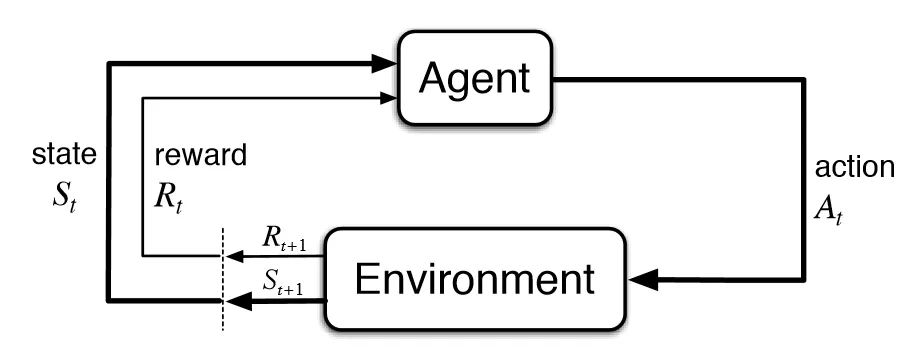
\includegraphics[width=0.6\textwidth]{Images/AgentEnvironment.png}
\caption{Interaction between the agent and the environment in Reinforcement Learning \cite{sutton_reinforcement_2018}.}
\label{Figure:AgentEnvironment}
\end{figure}

The goal of the agent is to maximise the return. The return is the discounted sum of the rewards the agent collects from time \( t \) onwards \cite{sutton_reinforcement_2018}:

\begin{equation}
R_{t+1} + \gamma R_{t+2} + \gamma^2 R_{t+3} + \ldots = \sum_{k=0}^{\infty} \gamma^k R_{t+k+1}
\end{equation}

Here, \( \gamma \) is the discount factor. It sets how much future rewards count compared with immediate ones. A policy \( \pi \) decides the actions of the agent. It can be deterministic, giving one specific action for each state, or stochastic, giving a probability distribution over actions. A main difficulty in RL is the balance between exploration and exploitation. Exploration means trying new actions to find out their effects. Exploitation means choosing actions that are known to give a high reward. A common approach is the \(\varepsilon\)-greedy policy, which usually picks the best-known action but sometimes picks a random one \cite{sutton_reinforcement_2018}. This method needs a discrete set of actions, because it works by picking one of the alternatives at random. When the action is continuous, as in this work, exploration comes instead from adding noise to the action the policy returns. \Cref{Section:DeepReinforcementLearning} describes this approach together with the algorithm that uses it.

Reinforcement Learning is built on the Markov Decision Process (MDP), defined by the tuple \( (S, A, P, R, \gamma) \). Here, \( S \) is the set of all possible states of the environment and \( A \) is the set of actions the agent can take. \( P \) is the transition probability, the probability of moving from state \( s_t \) to state \( s_{t+1} \) after taking action \( a \). \( R \) is the reward function, which gives the reward for that transition, and \( \gamma \) is the discount factor. MDPs rely on the Markov property. It requires the next state to depend only on the current state and action, and not on any earlier ones \cite{sutton_reinforcement_2018}:

\begin{equation}
\label{Equation:MarkovProperty}
P(s_{t+1} | s_t, a_t, s_{t-1}, a_{t-1}, \ldots, s_0, a_0) = P(s_{t+1} | s_t, a_t)
\end{equation}

The reward function matters because it is where the goal of the task is defined. It tells the agent what to achieve, but not how to achieve it. The agent will adopt any behaviour that raises the reward. In trading, the reward is normally computed from profit and loss. This drives the agent towards profitable positions without telling it which positions those are \cite{sutton_reinforcement_2018}.

\subsection{Value Functions and Q-Functions}

The value function of a policy \( \pi \), written \( V^\pi(s) \), is the expected return when starting in state \( s \) and following policy \( \pi \) after that. It is defined as follows \cite{sutton_reinforcement_2018}:

\begin{equation}
V^\pi(s) = \mathbb{E} \left[ \sum_{k=0}^{\infty} \gamma^k R_{t+k+1} \mid S_t = s, \pi \right]
\end{equation}

Here, \( \gamma \) is the discount factor, which sets how much future rewards count compared with immediate rewards. \( \mathbb{E} \) is the expected value, the average of all possible outcomes weighted by their probabilities. The Q-function of a policy \( \pi \), written \( Q^\pi(s, a) \), is the expected return for taking action \( a \) in state \( s \) and following policy \( \pi \) after that. It is defined as follows \cite{sutton_reinforcement_2018}:

\begin{equation}
Q^\pi(s, a) = \mathbb{E} \left[ \sum_{k=0}^{\infty} \gamma^k R_{t+k+1} \mid S_t = s, A_t = a, \pi \right]
\end{equation}

The Bellman equations are named after Richard Bellman, who first formulated them. They give a recursive decomposition of the total cumulative reward an agent can expect, starting from a given state or state-action pair. These equations are the basis of dynamic programming methods in RL. They express the value of a state, or of a state-action pair, in terms of the values of the states that follow it. This recursion is what allows the estimated values to be improved step by step, and it is the basis of convergence for most RL algorithms. The equations are as follows \cite{sutton_reinforcement_2018}:

\begin{equation}
V^\pi(s) = \sum_{a \in A} \pi(a|s) \sum_{s' \in S} P(s'|s,a) \left[ R(s,a,s') + \gamma V^\pi(s') \right]
\end{equation}

\begin{equation}
Q^\pi(s, a) = \sum_{s' \in S} P(s'|s,a) \left[ R(s,a,s') + \gamma \sum_{a' \in A} \pi(a'|s') Q^\pi(s', a') \right]
\end{equation}

\begin{equation}
\label{Equation:RelationshipValueQFunction}
V^\pi(s) = \sum_{a \in A} \pi(a|s) Q^\pi(s, a)
\end{equation}

\Cref{Equation:RelationshipValueQFunction} shows that the value of a state under policy \(\pi\) is the expected value of the Q-function over all possible actions, weighted by the probability the policy gives to each action. For optimal policies, the optimal value function \( V^*(s) \) and the optimal Q-function \( Q^*(s, a) \) give the highest return that can be achieved from any state or state-action pair, respectively. From the Bellman equation, it follows that \cite{sutton_reinforcement_2018}:

\begin{equation}
V^*(s) = \max_{a \in A} \sum_{s' \in S} P(s'|s,a) \left[ R(s,a,s') + \gamma V^*(s') \right]
\end{equation}

\begin{equation}
Q^*(s, a) = \sum_{s' \in S} P(s'|s,a) \left[ R(s,a,s') + \gamma \max_{a' \in A} Q^*(s', a') \right]
\end{equation}

\begin{equation}
V^*(s) = \max_{a \in A} Q^*(s, a)
\end{equation}

By applying these equations again and again, RL algorithms gradually approximate the value function and the Q-function. This guides the agent towards the optimal policy, which is the policy that maximises the expected cumulative reward \cite{sutton_reinforcement_2018}.

\subsection{Methodological Variants and Learning Methods}

Reinforcement learning methods can be divided into groups by the properties of the learning method: model-based or model-free, on-policy or off-policy, and value-based or policy-based. In model-based RL, the algorithm builds a model of the environment to simulate and predict the outcomes of actions. The agent can then plan by predicting the next states. This is possible when the environment is simple enough to be modelled. In model-free RL, the algorithm learns a policy or a value function directly from its interactions with the environment, without building a model of it. Model-free methods are often chosen when the environment is hard to model or when no accurate model is available. Within model-free RL, there are on-policy methods, which learn about the policy that is currently used to make decisions, and off-policy methods, which explore with a different policy while they try to learn an optimal one \cite{sutton_reinforcement_2018}.

Another important distinction is between value-based methods, also called critic-only, and policy-based methods, also called actor-only. Value-based methods, such as Temporal Difference Learning (TD), Q-Learning and SARSA Learning, estimate the value of states or of state-action pairs. The policy is not learned directly. It follows from these values. Temporal Difference learning is the update rule that the other two are built on, and it works in both settings. SARSA is on-policy, because it evaluates the policy it is following. Q-Learning is off-policy, because it evaluates the greedy policy, the one that always takes the highest-valued action, whatever policy it actually follows. To take the highest-valued action, the method has to compare every action, so these methods are limited to discrete sets of actions. Policy-based methods, such as REINFORCE, optimise the policy directly. For this reason they extend to continuous actions, where the policy returns the action itself instead of a value for each possible action. Actor-Critic learning combines the two. It has a policy function (the actor) and a value function (the critic). The policy is improved directly, and the critic gives the value estimates that make those updates stable \cite{sutton_reinforcement_2018}. \Cref{Codes:ActorCritic} gives a detailed implementation.

% !TEX root = ../Main.tex
\begin{algorithm}[htb!]
\DontPrintSemicolon
\KwRequire{$\pi(a \mid s; \theta)$: a differentiable policy, $Q(s, a; w)$: a differentiable $Q$-function, $N$: number of iterations and learning rates $\beta^\theta > 0$ and $\beta^w > 0$}
Initialise policy parameter $\theta^{(0)}$ and $Q$-function parameter $w^{(0)}$\;
Initialise state $s$\;
\For{$n = 0, 1, \ldots, N - 1$}{
    Sample $a \sim \pi(\cdot \mid s; \theta^{(n)})$\;
    Take action $a$, observe state $s'$ and reward $r$\;
    Sample $a' \sim \pi(\cdot \mid s'; \theta^{(n)})$\;
    Compute the TD error: $\delta \gets r + \gamma Q(s', a'; w^{(n)}) - Q(s, a; w^{(n)})$\;
    Update $w$: $w^{(n+1)} \gets w^{(n)} + \beta^w \delta \nabla_w Q(s, a; w^{(n)})$\;
    Update $\theta$: $\theta^{(n+1)} \gets \theta^{(n)} + \beta^\theta \delta \nabla_\theta \ln \pi(a \mid s; \theta^{(n)})$\;
    $s \gets s'$\;
}
\caption{Actor-Critic \cite{sutton_reinforcement_2018}.}
\label{Codes:ActorCritic}
\end{algorithm}

For finite Markov Decision Processes, standard results guarantee that an optimal policy exists and that it can be taken to be deterministic and stationary. These guarantees do not extend to complex, non-stationary environments such as financial markets \cite{sutton_reinforcement_2018}. A raw price series does not have the Markov property. The information a trader uses is spread across the recent history, and is not all contained in the latest quote. RL applied to these markets therefore works with an approximation. Technical indicators and other engineered features put enough of that history into the state for the Markov property to hold approximately. Actor-Critic methods matter here because they are the point where reinforcement learning and neural networks meet. This is the subject of the next section.

% !TEX root = ../../Main.tex
\section{Deep Reinforcement Learning}
\label{Section:DeepReinforcementLearning}

Deep Reinforcement Learning (DRL) combines the decision making of reinforcement learning with the function approximation of neural networks. The value functions and policies of \Cref{Section:ReinforcementLearning} are defined over states. In a tabular setting, each state is stored separately, as one entry in a table. This is not possible when the state is a vector of continuous market variables, because there is no limit to the number of distinct states. Replacing the table with a neural network removes that limit. It also lets the agent generalise from states it has seen to states it has not seen.

\subsection{Fundamentals and History}

DRL appeared once it became clear that neural networks could serve as the function approximators that reinforcement learning needed to handle high-dimensional input. The result that started the field was the Deep Q-Network. It learned to play a range of Atari 2600 games directly from raw pixels and reached human-level scores on many of them \cite{mnih_playing_2013, mnih_human-level_2015}. It showed that a single architecture could learn control policies from raw, high-dimensional input, without features designed for each task. This result led to interest in applying the same methods to financial markets. There, the input is also high-dimensional, and the mapping from observation to decision is also unknown. However, an Atari game is stationary and fully observable, and a market is neither. For this reason, results carry over to markets much less directly than the comparison with games suggests.

\subsection{Deep Value-Based RL Algorithms: Deep Q-Networks}

Deep value-based methods use a neural network to approximate the Q-function. This lets them work with state spaces too large to list one by one. Neural Fitted Q Iteration was an early method of this kind. It fitted a network to the Q-values of a stored set of transitions, and fitted it again as more transitions were collected \cite{riedmiller_neural_2005}. The approach became established with the Deep Q-Network (DQN) algorithm \cite{mnih_human-level_2015}, which added two mechanisms that made training stable enough to be practical. The first is a separate target network. This is a delayed copy of the value network, used to compute the learning targets, so that the target does not move as fast as the estimate. The second is experience replay. This is a buffer of past transitions from which mini-batches are drawn at random, which breaks the temporal correlation between consecutive samples. The algorithm used in this work uses both mechanisms.

After DQN, the Double Deep Q-Network (DDQN) dealt with the tendency of DQN to overestimate action values \cite{van_hasselt_deep_2016}. It separates action selection from action evaluation. The online network, the one being trained, chooses the action, and the target network scores it. Deep value-based methods are not used in this work. They select an action by comparing the values of all available actions, and this requires the set of actions to be discrete.

\subsection{Deep Policy-Based RL Algorithms: Deep Policy Gradients}

Deep policy-based algorithms optimise the policy directly, without deriving it from action values. This is what allows them to work with continuous actions. In trading this matters, because a position has a size as well as a direction. A method limited to a discrete set of actions has to decide that size outside the learned policy. The Deep Deterministic Policy Gradient (DDPG) algorithm is a model-free, off-policy, actor-critic method for continuous action spaces \cite{lillicrap_continuous_2015}. It keeps four networks. The actor \( \mu(s | \theta^{\mu}) \) maps a state to a single action. The critic \( Q(s, a | \theta^{Q}) \) estimates the value of a state-action pair. The other two are delayed copies of these, the target actor \( \mu' \) and the target critic \( Q' \). Transitions are stored in a replay buffer, and mini-batches of \( N \) transitions are sampled from it at random. The critic is trained in the same way as in DQN. It minimises the squared error between its estimate and a target built from the observed reward and the value of the next state \cite{lillicrap_continuous_2015}:

\begin{equation}
y_i = r_i + \gamma \, Q'\!\left(s_{i+1}, \mu'(s_{i+1} | \theta^{\mu'}) \,\middle|\, \theta^{Q'}\right)
\label{Equation:DDPGTarget}
\end{equation}

\begin{equation}
L = \frac{1}{N} \sum_{i} \left( y_i - Q(s_i, a_i | \theta^{Q}) \right)^2
\label{Equation:DDPGCriticLoss}
\end{equation}

The actor is updated with the deterministic policy gradient, which follows the direction in which the value estimated by the critic increases. Because the action is continuous, the gradient of the value with respect to the action is defined, and the chain rule carries it back to the parameters of the actor \cite{lillicrap_continuous_2015}:

\begin{equation}
\nabla_{\theta^{\mu}} J \approx \frac{1}{N} \sum_{i} \nabla_{a} Q(s, a | \theta^{Q}) \big|_{s = s_i,\, a = \mu(s_i)} \; \nabla_{\theta^{\mu}} \mu(s | \theta^{\mu}) \big|_{s_i}
\label{Equation:DeterministicPolicyGradient}
\end{equation}

The target networks are not simply copied from the trained networks. After every update, they are moved a small fraction \( \tau \ll 1 \) towards them. This keeps the learning targets almost stationary, but it also slows down how fast they follow improvements \cite{lillicrap_continuous_2015}:

\begin{equation}
\theta' \leftarrow \tau \theta + (1 - \tau) \theta'
\label{Equation:SoftUpdate}
\end{equation}

The policy is deterministic, so it does not explore by itself, and the exploration problem raised in \Cref{Section:ReinforcementLearning} comes back here. DDPG solves it by adding a noise process \( \mathcal{N} \) to the action during training, so the action actually executed is \( \mu(s | \theta^{\mu}) + \mathcal{N} \). The original work uses an Ornstein-Uhlenbeck process. This process gives noise that is correlated in time, instead of independent at each step. The reason given is that a physical system with momentum explores better when a disturbance lasts for a while than when it changes sign at every step \cite{lillicrap_continuous_2015}. \Cref{Codes:DeepDeterministicPolicyGradient} shows the complete procedure.

% !TEX root = ../Main.tex
\begin{algorithm}[htb!]
\DontPrintSemicolon
\KwRequire{an actor $\mu(s | \theta^{\mu})$, a critic $Q(s, a | \theta^{Q})$, a discount factor $\gamma$, a soft update rate $\tau \ll 1$ and a minibatch size $N$}
Randomly initialise the critic parameters $\theta^{Q}$ and the actor parameters $\theta^{\mu}$\;
Initialise the target parameters $\theta^{Q'} \leftarrow \theta^{Q}$ and $\theta^{\mu'} \leftarrow \theta^{\mu}$, and the replay buffer $\mathcal{B}$\;
\For{episode $= 1, M$}{
    Initialise a random process $\mathcal{N}$ for action exploration\;
    Receive the initial observation state $s_1$\;
    \For{$t = 1, T$}{
        Select the action $a_t = \mu(s_t | \theta^{\mu}) + \mathcal{N}_t$ from the current policy and the exploration noise\;
        Execute the action $a_t$ and observe the reward $r_t$ and the new state $s_{t+1}$\;
        Store the transition $(s_t, a_t, r_t, s_{t+1})$ in $\mathcal{B}$\;
        Sample a random minibatch of $N$ transitions $(s_i, a_i, r_i, s_{i+1})$ from $\mathcal{B}$\;
        Set $y_i = r_i + \gamma Q'(s_{i+1}, \mu'(s_{i+1} | \theta^{\mu'}) | \theta^{Q'})$\;
        Update the critic by minimising the loss: $L = \frac{1}{N}\sum_i (y_i - Q(s_i, a_i | \theta^{Q}))^2$\;
        Update the actor policy using the sampled policy gradient:\;
        $\nabla_{\theta^{\mu}} J \approx \frac{1}{N}\sum_i \nabla_a Q(s, a | \theta^{Q})|_{s = s_i, a = \mu(s_i)} \nabla_{\theta^{\mu}} \mu(s | \theta^{\mu})|_{s_i}$\;
        Update the target networks:\;
        $\theta^{Q'} \leftarrow \tau \theta^{Q} + (1 - \tau) \theta^{Q'}$\;
        $\theta^{\mu'} \leftarrow \tau \theta^{\mu} + (1 - \tau) \theta^{\mu'}$\;
    }
}
\caption{Deep Deterministic Policy Gradient \cite{lillicrap_continuous_2015}.}
\label{Codes:DeepDeterministicPolicyGradient}
\end{algorithm}

DDPG is powerful, but it is not reliable. It has no guarantee of convergence except under restrictive conditions. It is also known to be sensitive to its hyperparameters and to the random seed, so two runs of the same configuration can end with different policies. A market makes this worse. It is non-stationary and only partially observable, which means the agent does not see the full state, and the guarantees that apply to finite Markov Decision Processes do not hold. These limits belong to the method itself. They are not problems that can be fixed. \Cref{Chapter:ExperimentalResults} therefore reports how the results vary, instead of reporting a single run.

This work combines the four topics covered here. It needs a market to trade in, networks to approximate the functions involved, a reinforcement learning formulation of the trading decision, and an algorithm that solves it for continuous actions. Combining them is not new. Many published studies have already tried it.

Those studies differ in how they define the state, the action and the reward. They also differ in whether the agent pays any cost for trading. These choices decide whether a reported result would hold on a live account. This makes them the right basis for comparing the published studies and for placing this work among them.